\subparagraph{Задание 4.17 (2)}

\textbf{Условие}:
Сбросить программу по Ctrl-F2. По F7 выполнить первые 6 инструкций. Открыть окно Execution History. Отменить последние 3 шага.

\textbf{Решение}:

\begin{figure}[!htp]
    \centering
    \begin{minipage}{0.32\textwidth}
        \centering
        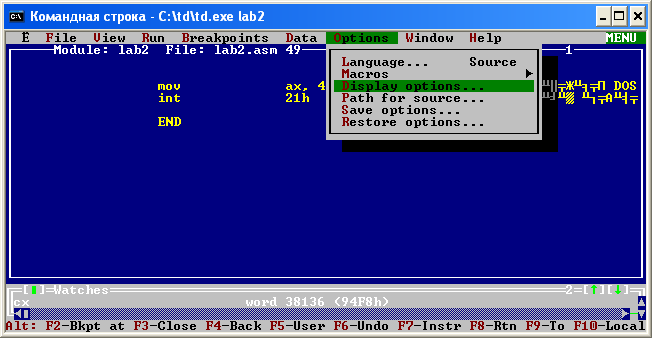
\includegraphics[width=.99\linewidth]
            {../_INCLUDES/task-4-17-2/1.png}
        \caption{1) }
        \label{fig:task_4_17_2__1}
    \end{minipage}
    \begin {minipage}{0.32\textwidth}
        \centering
        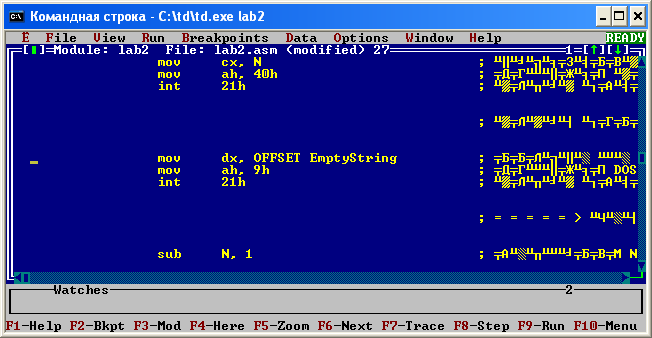
\includegraphics[width=.99\linewidth]
            {../_INCLUDES/task-4-17-2/2.png}
        \caption{2) }
        \label{fig:task_4_17_2__2}
    \end{minipage}
    \begin {minipage}{0.32\textwidth}
        \centering
        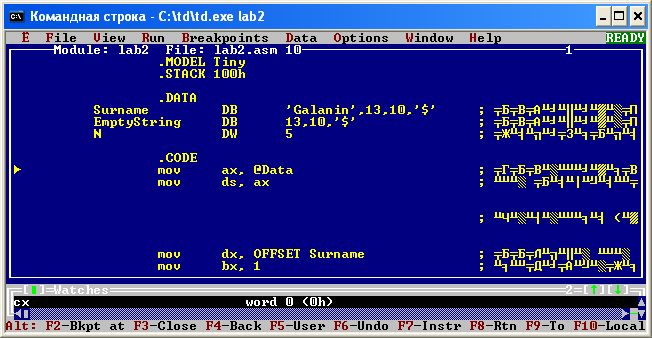
\includegraphics[width=.99\linewidth]
            {../_INCLUDES/task-4-17-2/3.png}
        \caption{3) }
        \label{fig:task_4_17_2__3}
    \end{minipage}
\end{figure}

В Turbo Debugger стрелка на строке \textbf{mov ax, @Data}.
Жму \textbf{F7}.
Рисунок~\ref{fig:task_4_17_2__1} (стр.~\pageref{fig:task_4_17_2__1}).

В Turbo Debugger стрелка на строке \textbf{mov ds, ax}.
Жму \textbf{F7}.
Рисунок~\ref{fig:task_4_17_2__2} (стр.~\pageref{fig:task_4_17_2__2}).

В Turbo Debugger стрелка на строке \textbf{mov dx, OFFSET Surname}.
Жму \textbf{F7}.
Рисунок~\ref{fig:task_4_17_2__3} (стр.~\pageref{fig:task_4_17_2__3}).

\begin{figure}[!htp]
    \centering
    \begin{minipage}{0.32\textwidth}
        \centering
        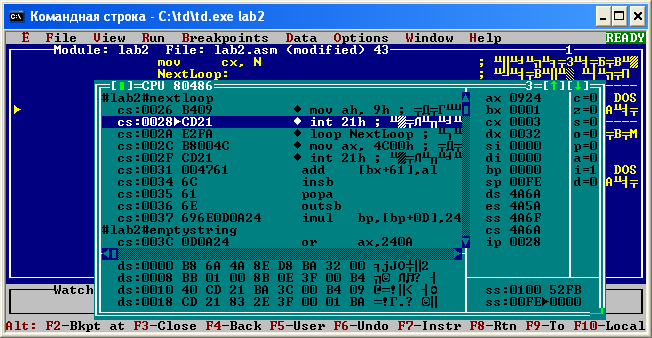
\includegraphics[width=.99\linewidth]
            {../_INCLUDES/task-4-17-2/4.png}
        \caption{4) }
        \label{fig:task_4_17_2__4}
    \end{minipage}
    \begin {minipage}{0.32\textwidth}
        \centering
        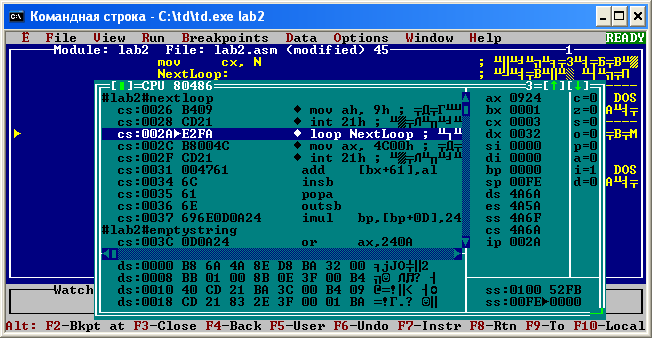
\includegraphics[width=.99\linewidth]
            {../_INCLUDES/task-4-17-2/5.png}
        \caption{5) }
        \label{fig:task_4_17_2__5}
    \end{minipage}
    \begin {minipage}{0.32\textwidth}
        \centering
        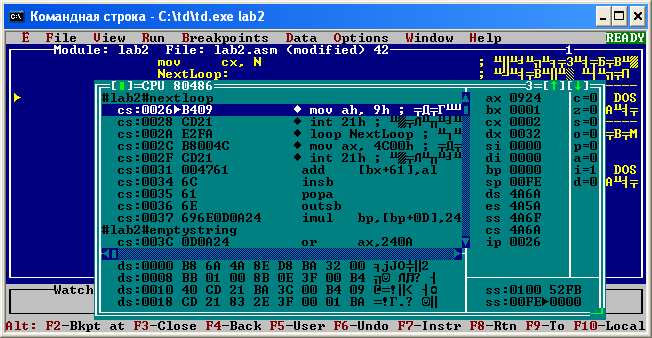
\includegraphics[width=.99\linewidth]
            {../_INCLUDES/task-4-17-2/6.png}
        \caption{6) }
        \label{fig:task_4_17_2__6}
    \end{minipage}
\end{figure}

В Turbo Debugger стрелка на строке \textbf{mov bx, 1}.
Жму \textbf{F7}.
Рисунок~\ref{fig:task_4_17_2__4} (стр.~\pageref{fig:task_4_17_2__4}).

В Turbo Debugger стрелка на строке \textbf{mov cx, N}.
Жму \textbf{F7}.
Рисунок~\ref{fig:task_4_17_2__5} (стр.~\pageref{fig:task_4_17_2__5}).

В Turbo Debugger стрелка на строке \textbf{mov ah, 40h}.
Жму \textbf{F7}.
Рисунок~\ref{fig:task_4_17_2__6} (стр.~\pageref{fig:task_4_17_2__6}).

\begin{figure}[!htp]
    \centering
    \begin{minipage}{0.32\textwidth}
        \centering
        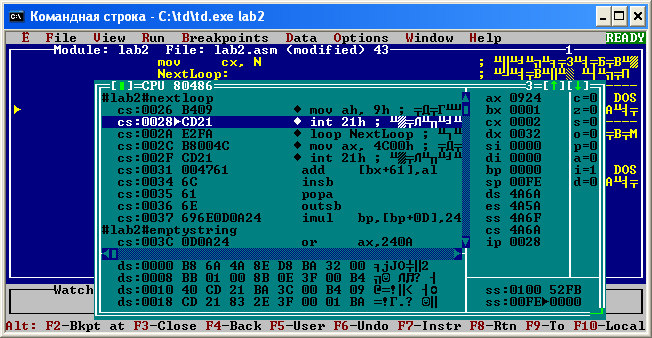
\includegraphics[width=.99\linewidth]
            {../_INCLUDES/task-4-17-2/7.png}
        \caption{7) }
        \label{fig:task_4_17_2__7}
    \end{minipage}
    \begin {minipage}{0.32\textwidth}
        \centering
        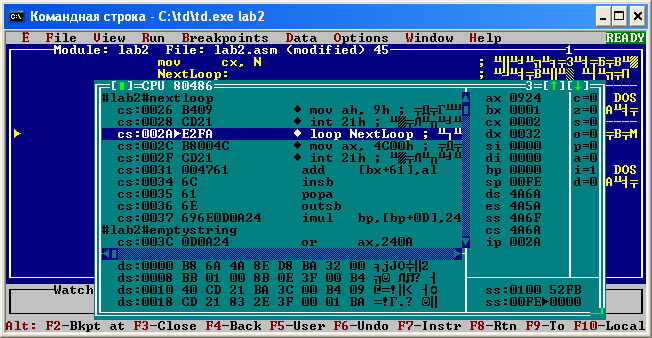
\includegraphics[width=.99\linewidth]
            {../_INCLUDES/task-4-17-2/8.png}
        \caption{8) }
        \label{fig:task_4_17_2__8}
    \end{minipage}
    \begin {minipage}{0.32\textwidth}
        \centering
        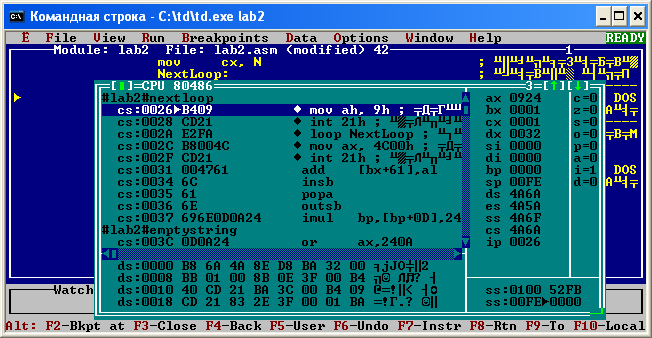
\includegraphics[width=.99\linewidth]
            {../_INCLUDES/task-4-17-2/9.png}
        \caption{9) }
        \label{fig:task_4_17_2__9}
    \end{minipage}
\end{figure}

В Turbo Debugger стрелка на строке \textbf{int 21h}.
Рисунок~\ref{fig:task_4_17_2__7} (стр.~\pageref{fig:task_4_17_2__7}).

Жму \textbf{F10} - попадаю в меню.
Выбираем пункт \textbf{View}.
Жму \textbf{Enter}.
Выбираем пункт \textbf{Execution history}.
Жму \textbf{Enter}.
Рисунок~\ref{fig:task_4_17_2__8} (стр.~\pageref{fig:task_4_17_2__8}).

Открылось осно с историей.
Предыдущая строка в истории \textbf{mov ah,40}.
Жмём \textbf{Alt} + \textbf{F4}.
Рисунок~\ref{fig:task_4_17_2__9} (стр.~\pageref{fig:task_4_17_2__9}).

\begin{figure}[!htp]
    \centering
    \begin{minipage}{0.32\textwidth}
        \centering
        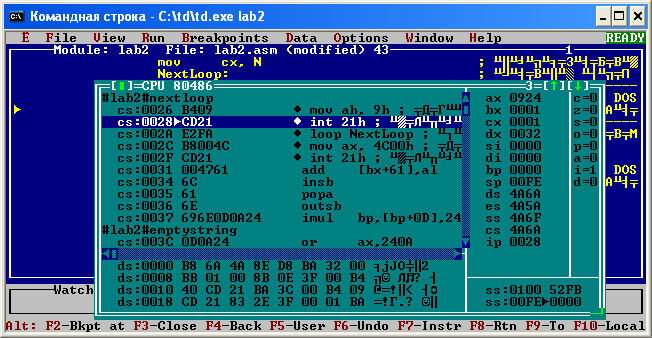
\includegraphics[width=.99\linewidth]
            {../_INCLUDES/task-4-17-2/10.png}
        \caption{10) }
        \label{fig:task_4_17_2__10}
    \end{minipage}
    \begin {minipage}{0.32\textwidth}
        \centering
        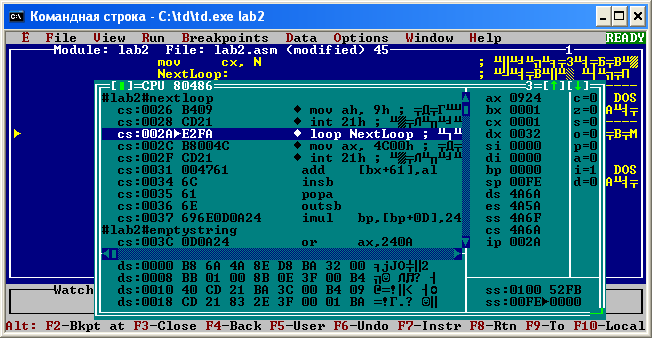
\includegraphics[width=.99\linewidth]
            {../_INCLUDES/task-4-17-2/11.png}
        \caption{11) }
        \label{fig:task_4_17_2__11}
    \end{minipage}
    \begin {minipage}{0.32\textwidth}
        \centering
        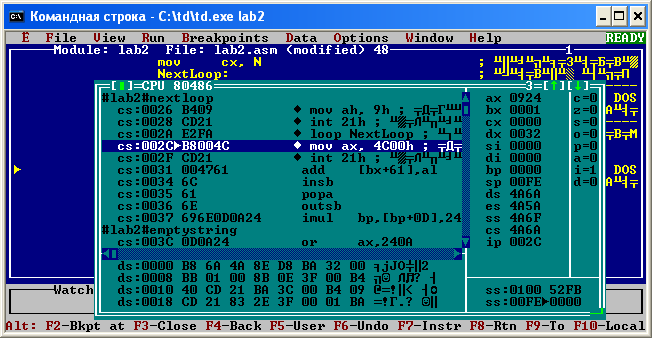
\includegraphics[width=.99\linewidth]
            {../_INCLUDES/task-4-17-2/12.png}
        \caption{12) }
        \label{fig:task_4_17_2__12}
    \end{minipage}
\end{figure}

Предыдущая строка в истории \textbf{mov cx, N}.
Жмём \textbf{Alt} + \textbf{F4}.
Рисунок~\ref{fig:task_4_17_2__10} (стр.~\pageref{fig:task_4_17_2__10}).

Предыдущая строка в истории \textbf{mov bx, 1}.
Жмём \textbf{Alt} + \textbf{F4}.
Рисунок~\ref{fig:task_4_17_2__11} (стр.~\pageref{fig:task_4_17_2__11}).

Предыдущая строка в истории \textbf{mov dx, OFFSET Surname}.
Рисунок~\ref{fig:task_4_17_2__12} (стр.~\pageref{fig:task_4_17_2__12}).
